\documentclass[a4paper]{article} 
\addtolength{\hoffset}{-2.25cm}
\addtolength{\textwidth}{4.5cm}
\addtolength{\voffset}{-3.25cm}
\addtolength{\textheight}{5cm}
\setlength{\parskip}{0pt}
\setlength{\parindent}{0in}

%----------------------------------------------------------------------------------------
%	PACKAGES AND OTHER DOCUMENT CONFIGURATIONS
%----------------------------------------------------------------------------------------

\usepackage{blindtext} % Package to generate dummy text
\usepackage{charter} % Use the Charter font
\usepackage[utf8]{inputenc} % Use UTF-8 encoding
\usepackage{microtype} % Slightly tweak font spacing for aesthetics
\usepackage[english, ngerman]{babel} % Language hyphenation and typographical rules
\usepackage{amsthm, amsmath, amssymb} % Mathematical typesetting
\usepackage{float} % Improved interface for floating objects
\usepackage[final, colorlinks = true, 
            linkcolor = black, 
            citecolor = black]{hyperref} % For hyperlinks in the PDF
\usepackage{graphicx, multicol} % Enhanced support for graphics
\usepackage{xcolor} % Driver-independent color extensions
\usepackage{marvosym, wasysym} % More symbols
\usepackage{rotating} % Rotation tools
\usepackage{censor} % Facilities for controlling restricted text
\usepackage{listings, style/lstlisting} % Environment for non-formatted code, !uses style file!
\usepackage{pseudocode} % Environment for specifying algorithms in a natural way
\usepackage{style/avm} % Environment for f-structures, !uses style file!
\usepackage{booktabs} % Enhances quality of tables
\usepackage{tikz-qtree} % Easy tree drawing tool
\tikzset{every tree node/.style={align=center,anchor=north},
         level distance=2cm} % Configuration for q-trees
\usepackage{style/btree} % Configuration for b-trees and b+-trees, !uses style file!
\usepackage[backend=biber,style=numeric,
            sorting=nyt]{biblatex} % Complete reimplementation of bibliographic facilities
\addbibresource{ecl.bib}
\usepackage{csquotes} % Context sensitive quotation facilities
\usepackage[yyyymmdd]{datetime} % Uses YEAR-MONTH-DAY format for dates
\renewcommand{\dateseparator}{-} % Sets dateseparator to '-'
\usepackage{fancyhdr} % Headers and footers
\pagestyle{fancy} % All pages have headers and footers
\fancyhead{}\renewcommand{\headrulewidth}{0pt} % Blank out the default header
\fancyfoot[L]{} % Custom footer text
\fancyfoot[C]{} % Custom footer text
\fancyfoot[R]{\thepage} % Custom footer text
\newcommand{\note}[1]{\marginpar{\scriptsize \textcolor{red}{#1}}} % Enables comments in red on margin

%----------------------------------------------------------------------------------------

\begin{document}

%-------------------------------
%	TITLE SECTION
%-------------------------------

\fancyhead[C]{}
\hrule \medskip % Upper rule
\begin{minipage}{0.295\textwidth} 
\raggedright
\footnotesize
\textbf{Pedro Luis Lobato Barros} \hfill\\    
202012490\hfill\\
p.lobato

\textbf{Jaime Andres Torres Bermejo} \hfill\\   
202014866\hfill\\
j.torres16

\textbf{Sofia Torres Ramírez} \hfill\\   
202014872\hfill\\
s.torres21

\end{minipage}
\begin{minipage}{0.4\textwidth} 
\centering 
\large 
Caso 1\\ 
\normalsize 
Infraestructura Computacional - Universidad de los Andes\\ 
\end{minipage}
\begin{minipage}{0.295\textwidth} 
\raggedleft
\today\hfill\\
\end{minipage}
\medskip\hrule 
\bigskip

%-------------------------------
%	CONTENTS
%-------------------------------

\section{Estructura del Proyecto}
    
    \subsection{UML}
    Por medio de este diagrama UML se puede entender a grandes rasgos el funcionamiento del programa. Iniciando por la clase “Process” Podemos ver que esta clase extiende de “Runnable”.  Siguiendo con esta Idea, las clases “Orange”, “Blue” y “Red” al representar los diferentes procesos que puede tener el programa implementarán a la clase “Process”. Tal como lo evidencia el diagrama, las clases “Orange” y “Blue” tienen el mismo objetivo final, procesar productos. Sin embargo, su funcionamiento interno es diferente y este se especificará más adelante. Los atributos de estas clases son:  
    
    \begin{enumerate}
        \item “msgLimit”: El número de productos o mensajes que se deben crear por cada tipo de proceso y que por ende se deben imprimir al finalizar el programa. Este atributo es estático por lo tanto está subrayado y solo se puede leer, no modificar.  
        \item “Id”: El identificador de cada proceso creado. 
        \item “stage”: El identificador de la etapa en la cual se encuentra el proceso creado. 
        \item “timeMillis”: El tiempo que debe dormir el proceso para simular la modificación del mensaje/producto. 
    \end{enumerate}
    Estos 4 atributos son iguales tanto para el proceso azul como para el naranja. El proceso rojo no tiene los atributos “stage”, “id” y “timeMillis” debido a que solo se crea un proceso rojo, el cual no necesitaría un id para diferenciarse. Se sabe que estará en la parte final del proceso por ende no es necesario especificar su etapa y al no modificar el mensaje no necesita un tiempo durante el cual simular esta modificación. Sin embargo, tiene un atributo adicional llamado “process” el cual tiene la información de cuantos procesos están activos. 

    Con respecto a la clase “Buffer” podemos ver que tiene los siguientes atributos: 
    \begin{enumerate}
        \item “MAX_SIZE”: La capacidad del buffer. 

        \item “queueOrange”: Una cola que almacena los productos/mensajes que fueron creados y modificados por procesos naranjas. 
        
        \item “queueBlue”: Una cola que almacena los productos/mensajes que fueron creados y modificados por procesos azules. 
        
        \item “occupied”: La cantidad de productos/mensajes que hay en el buffer. 
    \end{enumerate}
     

    Tanto el proceso naranja (Orange) como el azul (Blue) tienen dos relaciones con el Buffer. Una de estas relaciones representa el buffer de entrada, es decir, el Buffer del cual se sacan los mensajes para modificarlos. La cardinalidad de estas relaciones es de 0..1 debido a que si el proceso corresponde a la etapa 0, no existiría buffer de entrada ya que en esta etapa se crean los procesos. De lo contrario, es decir, si un proceso no pertenece al la etapa 0, siempre existirá un “Buffer in” del cual sacar los mensajes. Por otro lado, para todo proceso Azul o Naranja siempre existirá un “Buffer out” o Buffer de salida, en el cual se colocarán los mensajes ya modificados o recién creados para que un proceso de la siguiente etapa lo pueda coger y modificar. 

    Sin embargo, el proceso rojo no funciona igual debido a que este proceso solo tendrá interacción con el último Buffer, del cual sacará los mensajes para luego imprimirlos. 



    \subsection{la clase 'Main'}

    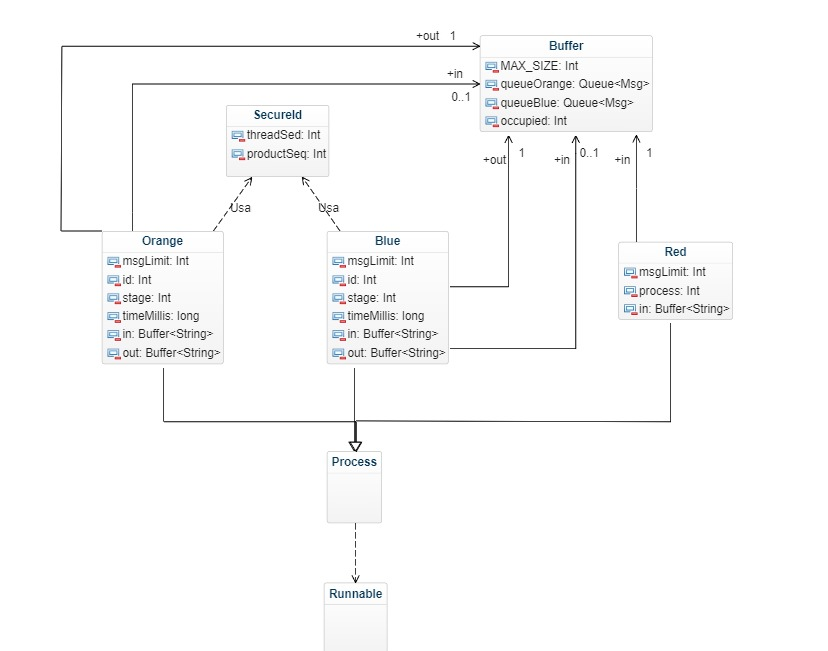
\includegraphics{uml.jpeg}

    La principal función de la clase 'Main', además de correr el programa,
    es unir al resto del programa para su funcionamiento óptimo, en 'Main.java'
    esta definida la estructura que las clases que vamos a manejar para solucionar
    el problema.

    Una de las primeras cosas que van a saltar a la vista es el uso de constantes
    definidas como 'final' dentro de la lógica de java. con esto, pretendemos 
    hacer que las variables acá definidas sean inmutables y no puedan ser cambiadas
    ni por el usuario ni por ninguno de los procesos que el programa corra una vez
    definidas. Las variables que caen dentro de este conjunto inmutable son

    \begin{enumerate}
        \item texttt{MESSAGE NUM:} Define el número de mensajes a enviar.
        \item texttt{PROCESS NUM:} Define el número de procesos del programa.
        \item texttt{BUFFER CAP:} Define el limite del Buffer
        \item texttt{BUFFER NUM:} Define el número de Buffers
        \item texttt{STAGE NUM:} Define el número de etapas por las que pasarán los procesos
    \end{enumerate}

    Estas conses son luego utilizadas para la creación de los objetos
    que serán usados en el programa, y conectará la lógica de esos
    nuevos objetos creados. 

    \subsection{Estructura de los Procesos}
    \subsubsectionmark{Blue}
    En la parte inicial del código se puede ver la definición de los atributos de la clase “Blue”, su método constructor y un método para darle valor al atributo “msgLimit”. 
    \subsection{Estructura de Input}
    
    \subsection{Estructura de Prints}
    
%------------------------------------------------

\section{Pruebas del programa}

\subsection{Estructura y requerimientos de prueba.}
Este programa fue probado en el IDE integrado IntelliJ IDEA 2022.3.2, con
el JDK Java 11 y en la consola integrada del IDE. Fue probado en Windows 10 
2H22 y Manjaro Linux 22.10, la estructura del proyecto esta planteada con el
sistema de Build 'Maven' y es dependiente principalmente de las librerías estandar
de Java. Sin embargo, para conseguir los prints con símbolos integrados, la fuente
de la consola en la cuál se compile debe ser compatible con simbolos Unicode,
de lo contrario, solo será mostrado el código Unicode referente a los símbolos.

\subsection{Pruebas}
\subsubsection{10-10-10}
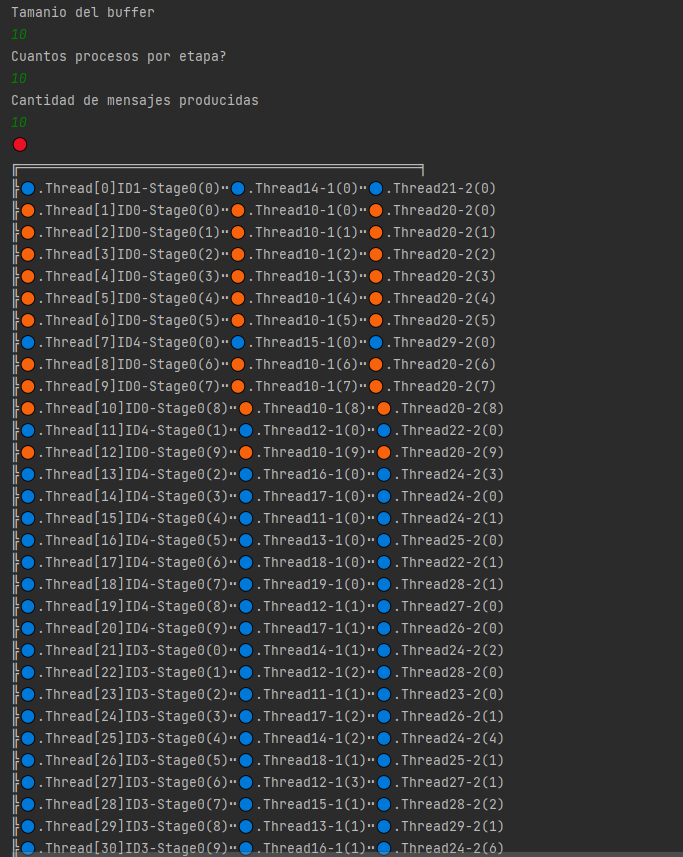
\includegraphics{10-10-10.PNG}

\subsubsection{3-3-3}
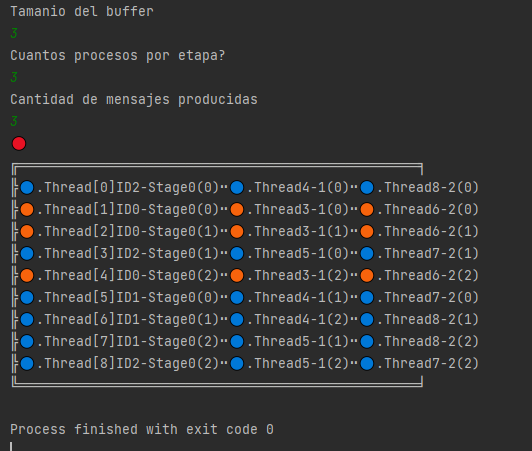
\includegraphics{3-3-3.PNG}

\subsubsection{5-5-5}
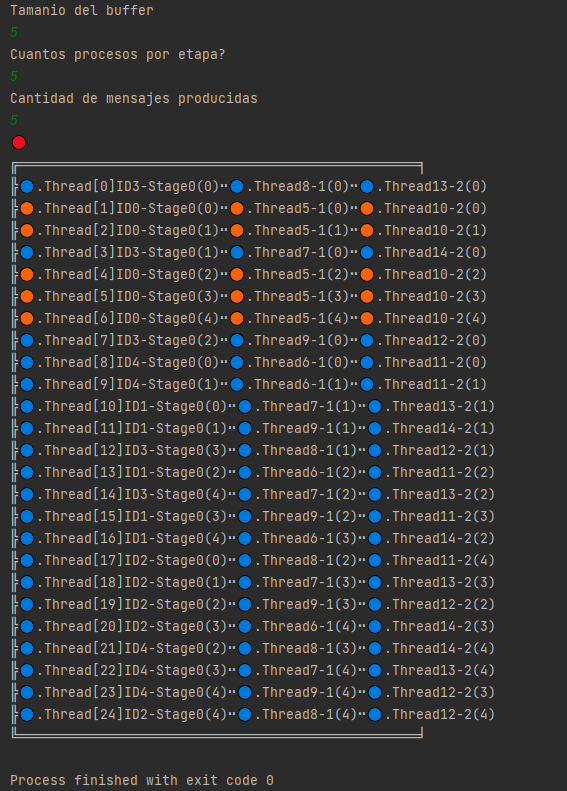
\includegraphics{5-5-5.PNG}

\section{Glosario}
\paragraph{Función Lambda}

\paragraph{Objeto anónimo}


%------------------------------------------------
\end{document}
